%-----------------------------------------------------------------------------%
\chapter{\babDua}
%-----------------------------------------------------------------------------%
% \lipsum[3-3]

%-----------------------------------------------------------------------------%
\section{Sejarah Singkat Perusahaan}
%-----------------------------------------------------------------------------%

% \lipsum[4-5]
\begin{figure}[H]
    \centering
    
\includegraphics[width=0.8\textwidth]{assets/pics/conciseLogo.png}
    \caption{Logo perusahaan PT Ganda Visi Jayatama}
    \label{concise-logo}
\end{figure}

Berdasarkan dokumen internal dari Universitas Multimedia Nusantara \cite{umn2023}, 
PT Ganda Visi Jayatama merupakan sebuah perusahaan yang bergerak di bidang IT Consultant 
yang sebelumnya berlokasi di Ruko Golden 8 Blok K No. 25. Hingga saat ini, perusahaan 
telah beroperasi selama kurang lebih 3 tahun dan kini bertempat di Ruko Crystal No. 19 
Gading Serpong. Selama periode tersebut, PT Ganda Visi Jayatama mengalami pertumbuhan 
pesat dengan memiliki sekitar 20 karyawan dari berbagai divisi. 

Perusahaan ini telah menyelesaikan berbagai proyek hingga tahun 2024, seperti Legal 
TINA, Spectacle, Kecap Inggeris, Home Mart, PMI Company Profile, dan Habco Company 
Profile. Saat ini, PT Ganda Visi Jayatama tengah mengerjakan beberapa proyek, di 
antaranya Habco MRO Apps, PMI Autopos, Enigma, dan proyek-proyek lainnya.


% Contoh sitasi lainnya menggunakan \verb|\cite| adalah saat kita mau mensitasi pekerjaan tentang \textit{Expert System} \cite{Djong2023AMethod} \textit{Blockchain} \cite{Christyono2021}, \textit{Fuzzy model} \cite{Widjaja2012}, \textit{machine learning} \cite{jain:2004} dan \textit{Dynamic Programming} \cite{bellman:1962}. Dokumen \latex~sangat mudah, seperti halnya membuat dokumen teks biasa. Ada 
% beberapa perintah yang diawali dengan tanda '\bslash'. 
% Seperti perintah \bslash\bslash~yang digunakan untuk memberi baris baru. 
% Perintah tersebut juga sama dengan perintah \bslash newline. 
% Pada bagian ini akan sedikit dijelaskan cara manipulasi teks dan 
% perintah-perintah \latex~yang mungkin akan sering digunakan. 
% Jika ingin belajar hal-hal dasar mengenai \latex, silahkan kunjungi: 

% \begin{itemize}
% 	\item \url{http://frodo.elon.edu/tutorial/tutorial/}, atau
% 	\item \url{http://www.maths.tcd.ie/~dwilkins/LaTeXPrimer/}
% \end{itemize}

% \cite{Marszaek2014ModelingCandlesticks}
%-----------------------------------------------------------------------------%
\section{Visi dan Misi Perusahaan}
%-----------------------------------------------------------------------------%

Visi dari PT Ganda Visi Jayatama adalah ”to be the go-to IT consultancy firm
for businesses looking to navigate the digital landscape with ease and confidence.”
Sedangkan misi dari perusahaan ini adalah ”to empower our clients by providing
personalized IT solutions that enable them to streamline operations, enhance
customer experiences, and drive growth. We accomplish this by staying at the
forefront of technology trends, adhering to industry best practices, and leveraging
a team of skilled and dedicated IT professionals. Ultimately, our goal is to help our
clients succeed in an ever-changing digital world.”

% Agar dapat menggunakan \latex~(pada konteks hanya sebagai pengguna), Anda 
% tidak perlu banyak tahu mengenai hal-hal di dalamnya. 
% Seperti halnya pembuatan dokumen secara visual (contohnya Open Office (OO) 
% Writer), Anda dapat menggunakan \latex~dengan cara yang sama. 
% Orang-orang yang menggunakan \latex~relatif lebih teliti dan terstruktur 
% mengenai cara penulisan yang dia gunakan, \latex~memaksa Anda untuk seperti itu.  

% Kembali pada bahasan utama, untuk mencoba \latex~Anda cukup men-\textit{download} 
% kompiler dan IDE. Saya menyarankan menggunakan Texlive dan Texmaker. 
% Texlive dapat di-\textit{download} dari \url{http://www.tug.org/texlive/}. 
% Sedangkan Texmaker dapat di-\textit{download} dari 
% \url{http://www.xm1math.net/texmaker/}. 
% Untuk pertama kali, coba buka berkas thesis.tex dalam template yang Anda miliki 
% pada Texmaker. 
% Dokumen ini adalah dokumen utama. 
% Tekan F6 (PDFLaTeX) dan Texmaker akan mengkompilasi berkas tersebut menjadi 
% berkas PDF. 
% Jika tidak bisa, pastikan Anda sudah meng-\textit{install} Texlive. 
% Buka berkas tersebut dengan menekan F7. 
% Hasilnya adalah sebuah dokumen yang sama seperti dokumen yang Anda baca saat ini. 


%-----------------------------------------------------------------------------%
\section{Struktur Organisasi Perusahaan}
%-----------------------------------------------------------------------------%
% Hal pertama yang mungkin ditanyakan adalah bagaimana membuat huruf tercetak 
% tebal, miring, atau memiliki garis bawah. 
% Pada Texmaker, Anda bisa melakukan hal ini seperti halnya saat mengubah dokumen 
% dengan OO Writer. 
% Namun jika tetap masih tertarik dengan cara lain, ini dia: 

% \begin{itemize}
% 	\item \bo{Bold} \\
% 		Gunakan perintah \bslash textbf$\lbrace\rbrace$ atau 
% 		\bslash bo$\lbrace\rbrace$. 
% 	\item \f{Italic} \\
% 		Gunakan perintah \bslash textit$\lbrace\rbrace$ atau 
% 		\bslash f$\lbrace\rbrace$. 
% 	\item \underline{Underline} \\
% 		Gunakan perintah \bslash underline$\lbrace\rbrace$.
% 	\item $\overline{Overline}$ \\
% 		Gunakan perintah \bslash overline. 
% 	\item $^{superscript}$ \\
% 		Gunakan perintah \bslash $\lbrace\rbrace$. 
% 	\item $_{subscript}$ \\
% 		Gunakan perintah \bslash \_$\lbrace\rbrace$. 
% \end{itemize}

% Perintah \bslash f dan \bslash bo hanya dapat digunakan jika package 
% uithesis digunakan untuk panduan. 

Struktur organisasi perusahaan PT Ganda Visi Jayatama dapat dilihat pada Gambar \ref{fig:struktur_organisasi}.

% %-----------------------------------------------------------------------------%
% \section{Memasukan Gambar}
% %-----------------------------------------------------------------------------%
% Setiap gambar dapat diberikan caption dan diberikan label. Label dapat 
% digunakan untuk menunjuk gambar tertentu. 
% Jika posisi gambar berubah, maka nomor gambar juga akan diubah secara 
% otomatis. 
% Begitu juga dengan seluruh referensi yang menunjuk pada gambar tersebut. 
% Contoh sederhana adalah \pic~\ref{fig:testGambar}. 
% Silahkan lihat code \latex~dengan nama bab2.tex untuk melihat kode lengkapnya. 
% Harap diingat bahwa caption untuk gambar selalu terletak dibawah gambar. 

\begin{figure}
	\centering
	\fbox{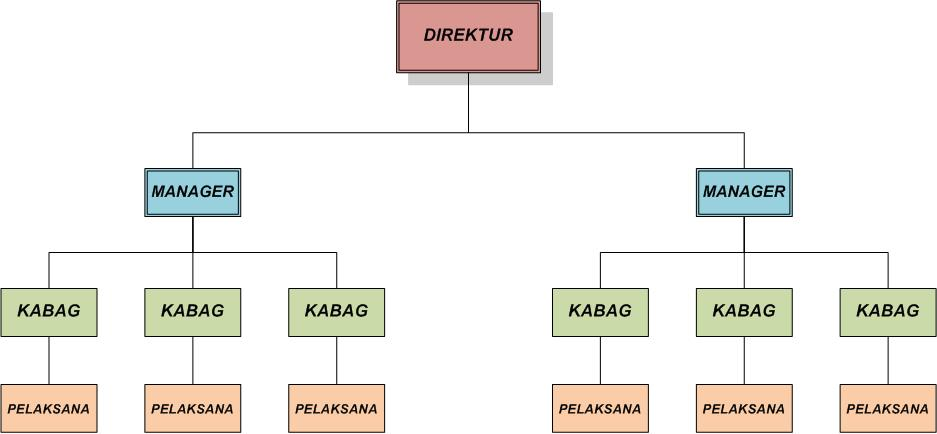
\includegraphics[width=0.90\textwidth]{assets/pics/fig_struktur-organisasi.jpg}}
	\caption{Struktur organisasi perusahaan PT Visi Ganda Jayatama }
	\vspace{0em}
	% \vspace{-1em} %kalau 2 baris
	% {\small Sumber: \cite{Widjaja2002a}}
	\label{fig:struktur_organisasi}
\end{figure}


